% Kopfzeile beim Kapitelanfang:
\fancypagestyle{plain}{
%Kopfzeile links bzw. innen
\fancyhead[L]{\Large Vorlesung 18 (12.12.2013)}
%Kopfzeile rechts bzw. außen
\fancyhead[R]{}}
%Kopfzeile links bzw. innen
\fancyhead[L]{\Large Vorlesung 18 (12.12.2013)}
%Kopfzeile rechts bzw. außen
\fancyhead[R]{}
% **************************************************

\phantomsection
\addcontentsline{toc}{section}{Sätze über stetige Funktionen}
\section*{Sätze über stetige Funktionen}
Erinnerung: $f: D \to \R$ stetig in $x_0 \in D :\Lra$
$$\forall \eps > 0 \exists \delta > 0: |f(x)-f(x_0)| < \eps \forall x \in D \text{ mit } |x-x_0| < \delta$$
$$\Lra \forall (x_n) \subseteq D \text{ mit } x_n \to x_0: f(x_n) \to f(x_0)$$

\section{Zwischenwertsatz (ZWS)}\label{9.18}
Seien $a,b \in \R$ mit $a<b$ und $f: [a,b] \to \R$ stetig $\Ra f$ nimmt jeden Wert zwischen $f(a)$ und $f(b)$ an.\\
Das heißt: $\gamma$ zwischen $f(a)$ und $f(b) \Ra \exists x \in [a,b]: f(x)=\gamma$\nl
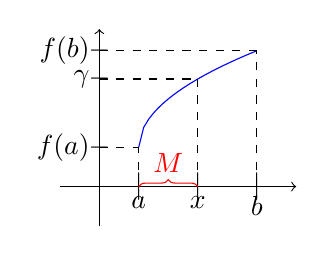
\begin{tikzpicture}
\draw[->] (-0.5,0)--(2.5,0);
\draw[->] (0,-0.5)--(0,2);
\draw[color=blue,domain=0.5:2] plot (\x, {sqrt(\x-0.5)+0.5});
\draw (0.5,0) node {$|$} node[below] {$a$};
\draw[dashed] (0.5,0)--(0.5,0.5);
\draw (2,0) node {$|$} node[below] {$b$};
\draw[dashed] (2,0)--(2,1.724744871);
\draw (0,0.5) node {$-$} node[left] {$f(a)$};
\draw[dashed] (0,0.5)--(0.5,0.5);
\draw (0,1.724744871) node {$-$} node[left] {$f(b)$};
\draw[dashed] (0,1.724744871)--(2,1.724744871);
\draw (1.25,0) node {$|$} node[below] {$x$};
\draw[dashed] (1.25,0)--(1.25,1.366025404);
\draw (0,1.366025404) node {$-$} node[left] {$\gamma$};
\draw[dashed] (0,1.366025404)--(1.25,1.366025404);
\draw[decoration={brace,mirror},decorate,color=red] (1.25,0)--(0.5,0);
\draw[color=red] (0.875,0.3) node {$M$};
\end{tikzpicture} \ 
\begin{tikzpicture}

\end{tikzpicture}

\subsection*{Beweis}
Sei etwa $f(a) \le f(b)$, o.E. $f(a) < \gamma < f(b)$\\
$M := \{t \in [a,b]: f(t) \le \gamma\}, M \neq \emptyset$ (da $a \in M$), beschränkt\\
$\Ra x := sum \ M$ existiert, $x \in [a,b]$\nl
\underline{Behauptung}: $f(x) = \gamma$\\
Dazu: $x = sum \ M \Ra \exists$ Folge $(t_n) \subseteq M: x - \frac{1}{n} < t_n \le x$\\
$\lim_{n \to \infty} t_n = x; f(t_n) \le \gamma$\\
$f$ stetig $\Ra f(x) = \lim f(t_n) \le \gamma < f(b)$, Insbes.: $x < b$\\
Wähle Folge $(s_n)$ in $(x,b]$ mit $s_n \to x$\\
$\Ra f(s_n) > \gamma$ (da $s_n \notin M$) und $f(x) = \lim f(s_n) \ge \gamma$ (Vergleichskriterium für Folgen, \ref{5.8}).\nl
\underline{Zus.}: $f(x) = \gamma$ \qed

\subsection*{Beispiel}
$f(x) = x + e^x - 2$ hat Nullstelle auf $[0,2]$\\
Denn: $f(0) = 1 - 2 < 0, f(2) = e^2 > 0$\\
$\underset{\text{ZWS}}{\Ra} \exists x \in [0,2]: f(x) = 0$

\newpage

\section{Satz: Nullstellen von Polynomen}\label{9.19}
Sei $p \in \Pow_\R$ ein reelles Polynom \underline{ungeraden} Grades.\\
$\Ra p$ hat mindestens eine reelle Nullstelle.\nl
\begin{tikzpicture}
\draw[->] (-2.5,0)--(2.5,0);
\draw[->] (0,-2.5)--(0,2.5);
\draw[color=blue,domain=-2.1:2.1] plot (\x, {0.25*(\x^3)});
\draw (-2,0) node {$|$} node[above] {$r$};
\draw (2,0) node{$|$} node[below] {$s$};
\draw (2,2) node{$\bullet$} node[right] {$P$};
\draw (-2,-2) node{$\bullet$};
\draw[dashed] (-2,0)--(-2,-2);
\draw[dashed] (2,0)--(2,2);
\end{tikzpicture}

\subsection*{Beweis}
$p$ habe o.E. Leitkoeffizienten $1$, das heißt $p(x) = x^n + a_{n-1} x^{n-1} + \ldots + a_0$\\
$\underset{x \neq 0}{=} x^n (\underbrace{1+\frac{a_{n-1}}{x} + \ldots + \frac{a_0}{x^n}}_{=: h(x)})$\\
$\lim_{x \to \pm \infty} h(x) = 1$\\
$\Ra \exists s > 0: h(s) > 0, \exists r < 0: h(r) > 0$\\
$\Ra p(s) = s^n \cdot h(s) > 0; p(r) = r^n \cdot h(r) < 0$ ($n$ ungerade)\\
ZWS (\ref{9.18}) $\Ra \exists x \in [r,s]: p(x) = 0$ \qed

\subsection*{Bezeichnung}\label{AbgeschlossenKompakt}
\en{
\item Ein abgeschlossenes, beschränktes Intervall $[a,b] \subseteq \R$ heißt auch \underline{kompakt}.
\item Eine Funktion $f: D \to \R$ heißt beschränkt $:\Ra \exists M > 0: |f(x)| \le M \forall x \in D$
}

\newpage

\section{Satz: Maximum und Minimum}\label{9.20}
Sei $[a,b] \subseteq \R$ ein kompaktes Intervall, $f: [a,b] \to \R$ stetig $\Ra \exists x_1, x_2 \in [a,b]$:\\
$\underbrace{f(x_1)}_{min \ f(x) \in [a,b]} \le f(x) \le \underbrace{f(x_2)}_{max \ f(x) \in [a,b]} \forall x \in [a,b]$\nl
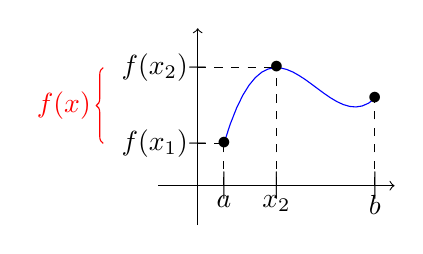
\begin{tikzpicture}
\draw[->] (-0.5,0)--(2.5,0);
\draw[->] (0,-0.5)--(0,2);
\draw[color=blue, domain=0.333333:2.25] plot (\x, {(\x-2)^3+1.5*(\x-2)^2+1});
\draw (0.333333,0) node {$|$} node[below] {$a$};
\draw (0.333333,0.5370359259) node {$\bullet$};
\draw[dashed] (0.333333,0)--(0.333333,0.5370359259);
\draw[dashed] (0,0.5370359259)--(0.333333,0.5370359259);
\draw (0,0.5370359259) node {$-$} node[left] {$f(x_1)$};
\draw (1,0) node {$|$} node[below] {$x_2$};
\draw (1,1.5) node {$\bullet$};
\draw[dashed] (1,0)--(1,1.5);
\draw[dashed] (0,1.5)--(1,1.5);
\draw (0,1.5) node {$-$} node[left] {$f(x_2)$};
\draw (2.25,0) node {$|$} node[below] {$b$};
\draw (2.25,1.109375) node {$\bullet$};
\draw[dashed] (2.25,0)--(2.25,1.109375);
\draw[decoration={brace,mirror},decorate,color=red] (-1.2,1.5)--(-1.2,0.5370359259);
\draw[color=red] (-1.7,1.018517963) node {$f(x)$};
\end{tikzpicture}

\subsection*{Beispiel (zu Notwendigkeit d. Vorauss.)}
\ena{
\item $f(x) = \frac{1}{x}$ auf $\underbrace{(0,1]}_{\text{nicht komp.!}}$, $f$ unbeschränkt\nl
\begin{tikzpicture}
\draw[->] (-0.5,0)--(2,0);
\draw[->] (0,-0.5)--(0,2);
\draw[color=blue,domain=0.5:1] plot (\x, {1/\x});
\draw (1,1) node {$\bullet$};
\draw[dashed] (1,0)--(1,1);
\draw (1,0) node {$|$} node[below] {$1$};
\draw (-0.3,-0.3) node {$0$};
\end{tikzpicture}
\item Auf $[0,1]: f(x) = \left\{\begin{array}{l} x, x \in [0,1) \\ 0, x = 1 \end{array}\right.$, $f$ unstetig, nimmt kein Maximum an.\nl
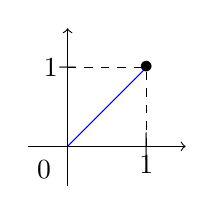
\begin{tikzpicture}
\draw[->] (-0.5,0)--(1.5,0);
\draw[->] (0,-0.5)--(0,1.5);
\draw[color=blue,domain=0:1] plot (\x, {\x});
\draw (1,1) node {$\bullet$};
\draw (1,0) node {$|$} node[below] {$1$};
\draw (0,1) node {$-$} node[left] {$1$};
\draw (-0.3,-0.3) node {$0$};
\draw[dashed] (0,1)--(1,1);
\draw[dashed] (1,0)--(1,1);
\end{tikzpicture}
}

\subsection*{Beweis}
Nachweis des Maximums (Minimum analog)\\
$s := sup\{f(x): x \in [a,b]\} \in \R \cup \{\pm \infty\}$ ($s := +\infty$, falls $f$ nach oben unbeschr.)\\
Def. von $sup \Ra \exists$ Folge $(x_n) \subseteq [a,b]: f(x_n) \to s$\\
$(x_n)$ beschränkt $\Ra$ (Bolzano-Weierstraß, \ref{5.12}) $(x_n)$ hat konv. Teilfolge $(s_{n_k})$.\\
Sei $x_{n_k} \to x \in \R$. $a \le x_{n_k} \le b \forall k \Ra a \le x \le b$\\
$f$ stetig $\Ra \underbrace{f(x_{n_k})}_{\to s \text{ wegen (*)}} \to f(x) \Ra s = f(x) < \infty \wedge s = \underset{x \in [a,b]}{max} \ f(x)$ \qed

\chapter{Monotone Funktionen und ihre Umkehrfunktion}\label{P10}
\section{Definition}\label{10.1}
Sei $D \subseteq \R; f: D \to \R$ heißt monoton wachsend [fallend] $:\Lra \forall x,y \in D$ mit $x<y$ gilt $f(x) \le f(y)$ [$f(x) \ge f(y)$]\\
Ist sogar stets $f(x) < f(y)$ [$f(x) > f(y)$], so heißt $f$ streng monoton wachsend [fallend].

\subsection*{Beispiel}
\en{
\item Potenzfunktion $x \mto x^k$ ($k \in \N$) streng monton wachsend (s.m.w.) auf $[0,\infty)$\nl
\begin{tikzpicture}
\draw[->] (-0.5,0)--(2,0);
\draw[->] (0,-0.5)--(0,3);
\draw[color=blue,domain=0:1.7320508] plot (\x, {\x^2});
\draw (-0.3,-0.3) node {$0$};
\draw (2,3) node {$x^k$};
\end{tikzpicture}
\item Floor-Funktion $x \mto \lfloor x \rfloor, x \in \R$ monoton wachsend, aber nicht streng monoton, nicht injektiv\nl
\begin{tikzpicture}
\draw[->] (-1,0)--(3,0);
\draw[->] (0,-2)--(0,3);
\draw[color=blue,domain=-1:3] plot (\x, {floor(\x)});
\draw (-0.3,-0.3) node {$0$};
\draw (1,-0.3) node {$1$};
\draw (2,-0.3) node {$2$};
\end{tikzpicture}
}

\newpage

\section{Lemma}\label{10.2}
Sei $f: D \to \R$ s.m.w. [s.m.f.] $\Ra f: D \to f(D) = \{f(x): x \in D\}$ ist bijektiv, und $f^{-1}: f(D) \to D$ ist s.m.w. [s.m.f.]\nl
\begin{tikzpicture}
\draw[->] (-3,0)--(3,0);
\draw[->] (0,-3)--(0,3);
\draw[color=blue,domain=-3:1.0986] plot (\x, {exp(\x)});
\draw[color=blue,domain=0.05:3] plot (\x, {ln(\x)});
\draw (1.4,3) node {$f^{-1}$};
\draw (3,1.4) node {$f$};
\draw[dashed] (-3,-3)--(3,3);
\end{tikzpicture}

\subsection*{Beweis}
$x < y \Lra f(x) < f(y)$ (*)\\
(zu ``$\La$'' ang.: $x \ge y \underset{\text{s.m.w.}}{\Ra} f(x) \ge f(y)$ \wspruch)\\
$\Ra f$ injektiv, also $f: D \to f(D)$ bijektiv und aus ``$\La$'' in (*): $f^{-1}$ s.m.w.

\section{Satz: Stetigkeit der Umkehrfunktion}\label{10.3}
Sei $f: [a,b] \to \R$ s.m.w. und \underline{stetig}.\\
$\Ra f: [a,b] \to [f(a),f(b)]$ bijektiv und $f^{-1}$ ist ebenfalls s.m.w. und auch stetig.

\subsection*{Beweis}
$f$ stetig $\underset{\text{ZWS}}{\Ra} f$ nimmt jeden Wert aus $[f(a),f(b)]$ an (und keine sonstigen wegen Monotonie).\\
Ferner: $f^{-1}: [f(a),f(b)] \to [a,b]$ s.m.w. (\ref{10.2})\nl
$f^{-1}$ stetig:\\
% TODO: Graph
Sei $y_0 \in [f(a),f(b)], y_0 = f(x_0)$\\
Hier: Fall $a < x_0 < b$ ($x_0 \in \{a,b\}$) analog)\\
Sei $\eps > 0$ gegeben, o.E. so klein, dass $(x_0 - \eps, x_0 + \eps) \subseteq [a,b]$\\
$\alpha := f(x_0-\eps), \beta := f(x_0+\eps)$\\
$\alpha < y_0 < \beta$ (für s.m.w.)\nl
Sei $y \in [\alpha,\beta] \underset{f^{-1} \text{ s.m.w}}{\Ra} \underbrace{f^{-1}(\alpha)}_{x_0-\eps} \le f^{-1}(y) \le \underbrace{f^{-1}(\beta)}_{x_0+\eps}$\\
$\Ra |f^{-1}(y) - \underbrace{f^{-1}(y_0)}_{=x_0}| < \eps \forall y \in [\alpha,\beta]$\\
$\Ra f^{-1}$ stetig in $y_0$ \qed

\section{Beispiel: Wurzel-Funktion}\label{10.4}
Sei $k \in \N$ fest. Potenzfunktion: $f(x)=x^k, [0,\infty) \to [0,\infty)$\\
$f$ stetig und s.m.w., $f$ auch bijektiv, denn:\\
$y \ge 0 \Ra \exists! x \ge 0: x^k = y$, nämlich $x=\sqrt[k]{y}$\\
Umkehrfunktion: $f^{-1}: x \mto \sqrt[k]{x}, [0,\infty) \to [0,\infty)$ $k$-te Wurzelfunktion.\nl
Streng monoton wachsend nach Lemma \ref{10.2}, außerdem stetig auf $[0,\infty)$, denn:\\
Sei $R > 0$ beliebig $\Ra f: [0,\sqrt[k]{R}] \to [0,R]$ bijektiv $\underset{\text{\ref{10.3}}}{\Ra} f^{-1}$ stetig auf $[0,R] \underset{R \text{ bel.}}{\Ra} f^{-1}$ ist $[0,\infty)$.\nl
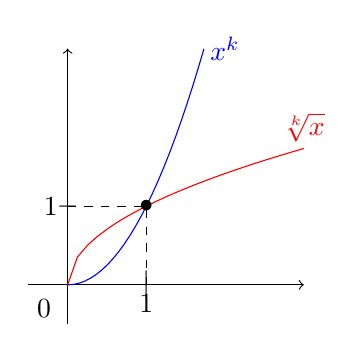
\begin{tikzpicture}
\draw[->] (-0.5,0)--(3,0);
\draw[->] (0,-0.5)--(0,3);
\draw[color=blue,domain=0:1.7320508] plot (\x, {\x^2});
\draw[color=red,domain=0:3] plot (\x, {sqrt(\x)});
\draw[color=blue] (2,3) node {$x^k$};
\draw[color=red] (3,2) node {$\sqrt[k]{x}$};
\draw (1,1) node {$\bullet$};
\draw (-0.3,-0.3) node {$0$};
\draw (1,0) node {$|$} node[below] {$1$};
\draw (0,1) node {$-$} node[left] {$1$};
\draw[dashed] (0,1)--(1,1);
\draw[dashed] (1,0)--(1,1);
\end{tikzpicture}